\documentclass[a4paper]{article}\usepackage[]{graphicx}\usepackage[]{color}
%% maxwidth is the original width if it is less than linewidth
%% otherwise use linewidth (to make sure the graphics do not exceed the margin)
\makeatletter
\def\maxwidth{ %
  \ifdim\Gin@nat@width>\linewidth
    \linewidth
  \else
    \Gin@nat@width
  \fi
}
\makeatother

\definecolor{fgcolor}{rgb}{0.345, 0.345, 0.345}
\newcommand{\hlnum}[1]{\textcolor[rgb]{0.686,0.059,0.569}{#1}}%
\newcommand{\hlstr}[1]{\textcolor[rgb]{0.192,0.494,0.8}{#1}}%
\newcommand{\hlcom}[1]{\textcolor[rgb]{0.678,0.584,0.686}{\textit{#1}}}%
\newcommand{\hlopt}[1]{\textcolor[rgb]{0,0,0}{#1}}%
\newcommand{\hlstd}[1]{\textcolor[rgb]{0.345,0.345,0.345}{#1}}%
\newcommand{\hlkwa}[1]{\textcolor[rgb]{0.161,0.373,0.58}{\textbf{#1}}}%
\newcommand{\hlkwb}[1]{\textcolor[rgb]{0.69,0.353,0.396}{#1}}%
\newcommand{\hlkwc}[1]{\textcolor[rgb]{0.333,0.667,0.333}{#1}}%
\newcommand{\hlkwd}[1]{\textcolor[rgb]{0.737,0.353,0.396}{\textbf{#1}}}%
\let\hlipl\hlkwb

\usepackage{framed}
\makeatletter
\newenvironment{kframe}{%
 \def\at@end@of@kframe{}%
 \ifinner\ifhmode%
  \def\at@end@of@kframe{\end{minipage}}%
  \begin{minipage}{\columnwidth}%
 \fi\fi%
 \def\FrameCommand##1{\hskip\@totalleftmargin \hskip-\fboxsep
 \colorbox{shadecolor}{##1}\hskip-\fboxsep
     % There is no \\@totalrightmargin, so:
     \hskip-\linewidth \hskip-\@totalleftmargin \hskip\columnwidth}%
 \MakeFramed {\advance\hsize-\width
   \@totalleftmargin\z@ \linewidth\hsize
   \@setminipage}}%
 {\par\unskip\endMakeFramed%
 \at@end@of@kframe}
\makeatother

\definecolor{shadecolor}{rgb}{.97, .97, .97}
\definecolor{messagecolor}{rgb}{0, 0, 0}
\definecolor{warningcolor}{rgb}{1, 0, 1}
\definecolor{errorcolor}{rgb}{1, 0, 0}
\newenvironment{knitrout}{}{} % an empty environment to be redefined in TeX

\usepackage{alltt}
\usepackage{graphicx}
\IfFileExists{upquote.sty}{\usepackage{upquote}}{}
\begin{document}
\title {Mediation}
\author{Erik Danay}

\maketitle
\section{Einf\"uhrung}
Eine kurze Einf\"uhrung zur Berechnung einer Mediation in
\texttt{lavaan} mit Angabe der Syntax. \par
Um eine Mediation durchzuf\"uhren, m\"ussen mehrere Schritte durchlaufen werden. 
\subsection{Variablen}
Zuerst m\"ussen \begin{itemize}
  \item Pr\"adiktor (X),   \item 
  Mediator (Z) und   \item 
  Kriterium (Y) 
\end{itemize}
klar zugeordnet werden.
Danach m\"ussen mit diesen drei Variablen verschiedene Modelle berechnet und miteinander verglichen werden. \par

\subsection{Modelle und Pfade}
Die Modelle unterscheiden sich dahingehend, welche Pfade \textit{zwischen} den Variablen eingezeichnet werden.
Die Pfade, die zwischen diesen drei Variablen stehen, werden spezifisch benannt:
\begin{itemize}
  \item Pfad von Pr\"adiktor (X) auf Kriterium (Y): \textbf{c
}  \item Pfad von Pr\"adiktor (X) auf Mediator (Z): \textbf{a}
\item Pfad von Mediator (Z) auf Kriterium (Y): \textbf{b}
\end{itemize}

Die Kombination aus Pfad a und Pfad b, also die Verbidung von Pr\"adiktor und Kriterium \"uber den Mediator, nennt man \texttt{indirekten Pfad}.
\begin{itemize}
  \item Pfad \textbf{a - b}: indirekter Pfad
\end{itemize}


Hier sind die drei Pfade in einem Gesamtmodell dargestellt:
\begin{figure}[ht]
\center
  \includegraphics[height=100pt]{/Users/lillion/Desktop/MEdiation.png}
  
  \caption{Mediation: volles Modell}
  \label{Mediation: volles Modell}
\end{figure}


\subsection{Drei Modell-Schritte}
\begin{enumerate}
  \item (Direktes Modell erstellen)
  \begin{enumerate}
  \item nicht unbedingt notwendig, da identisch der Korrelation von Pr\"adiktor und Kriterium
\end{enumerate}

  \item volles Modell erstellen
  \item indirektes Modell erstellen
\end{enumerate}

Man testet nun, ob das indirekte Modell, also das Modell des Mediators, nicht signifikant schlechter ist als das volle Modell. Ist dies der Fall, bedeutet das, dass der Pfad \"uber den Mediator, der sog. \texttt{indirekte Pfad}, die Aufkl\"arung der Varianz im Kriterium vollst\"andig \"ubernehmen kann.

Zuerst m\"ussen die notwendigen Pakete geladen werden. Hier im Beispiel zus\"atzlich noch der Datensatz

\begin{knitrout}
\definecolor{shadecolor}{rgb}{0.969, 0.969, 0.969}\color{fgcolor}\begin{kframe}
\begin{alltt}
\hlcom{# Daten}
\hlkwd{library}\hlstd{(umittr)}
\hlkwd{data}\hlstd{(crime_data)}
\hlstd{crime_data}\hlopt{$}\hlstd{crime} \hlkwb{<-} \hlstd{crime_data}\hlopt{$}\hlstd{crime}\hlopt{/}\hlnum{1000}
\hlcom{# Paket fuer SEM/Mediation}
\hlkwd{library}\hlstd{(lavaan)}
\end{alltt}


{\ttfamily\noindent\itshape\color{messagecolor}{\#\# This is lavaan 0.5-22}}

{\ttfamily\noindent\itshape\color{messagecolor}{\#\# lavaan is BETA software! Please report any bugs.}}\end{kframe}
\end{knitrout}

\subsection{Modellsyntax}
Danach muss das Modell spezifiziert werden. 

Die Syntax f\"ur Modelle folgt folgenden Vorgaben:

\begin{itemize}
  \item Modelle werden immer unter Anf\"uhrungszeichen per Syntax definiert: \textbf{' '}
  \item Man muss Modell mit \textbf{\textless-} einem Namen zuweisen wie im folgenden Beispiel: \texttt{modell \textless-'  '}
  \item Pfade sind innerhalb des Modells durch eine Tilde \textbf{\~ } symbolisiert. 
  \item Pfade benennt man dadurch, dass man vor die Variable \textbf{xyz*} schreibt.
\end{itemize}


\section{Modell erstellen}
\subsection{Modell 'zeichnen'}
Wir beginnen mit dem direkten Modell, der einfachen Korrelation.
\begin{knitrout}
\definecolor{shadecolor}{rgb}{0.969, 0.969, 0.969}\color{fgcolor}\begin{kframe}
\begin{alltt}
\hlcom{# Modell 1: (nur) direktes Modell}
\hlstd{Modelldirekt} \hlkwb{<-} \hlstr{'crime ~ pctwhite'}
\end{alltt}
\end{kframe}
\end{knitrout}

Das Modell liest man als: \textit{crime on pctwhite.}

Diese Modell stellt den direkten Pfad \textbf{c} dar. Man kann den \textbf{Pfad benennen}, wenn man die Syntax leicht erweitert und vor den Pr\"adiktor noch eine \textbf{Bezeichnung mit *} hinschreibt:
\begin{knitrout}
\definecolor{shadecolor}{rgb}{0.969, 0.969, 0.969}\color{fgcolor}\begin{kframe}
\begin{alltt}
\hlcom{# Modell 1: (nur) direktes Modell}
\hlstd{Modelldirekt} \hlkwb{<-} \hlstr{'crime ~ a * pctwhite'}
\end{alltt}
\end{kframe}
\end{knitrout}

\subsection{Modell graphisch darstellen}
Das Modell kann man sich schon graphisch ausgeben lassen.

\begin{knitrout}
\definecolor{shadecolor}{rgb}{0.969, 0.969, 0.969}\color{fgcolor}\begin{kframe}
\begin{alltt}
\hlcom{# Graphik leer}
\hlkwd{library}\hlstd{(semPlot)} \hlcom{# Graphikpaket aktivieren}
\hlkwd{semPaths}\hlstd{(Modelldirekt,} \hlkwc{style}\hlstd{=}\hlstr{"lisrel"}\hlstd{,}\hlkwc{nCharNodes} \hlstd{=} \hlnum{0}\hlstd{,} \hlkwc{whatLabels}\hlstd{=}\hlstr{"std"}\hlstd{,}\hlkwc{intercepts} \hlstd{= F,}\hlkwc{rotation}\hlstd{=}\hlnum{2}\hlstd{)}
\end{alltt}
\end{kframe}
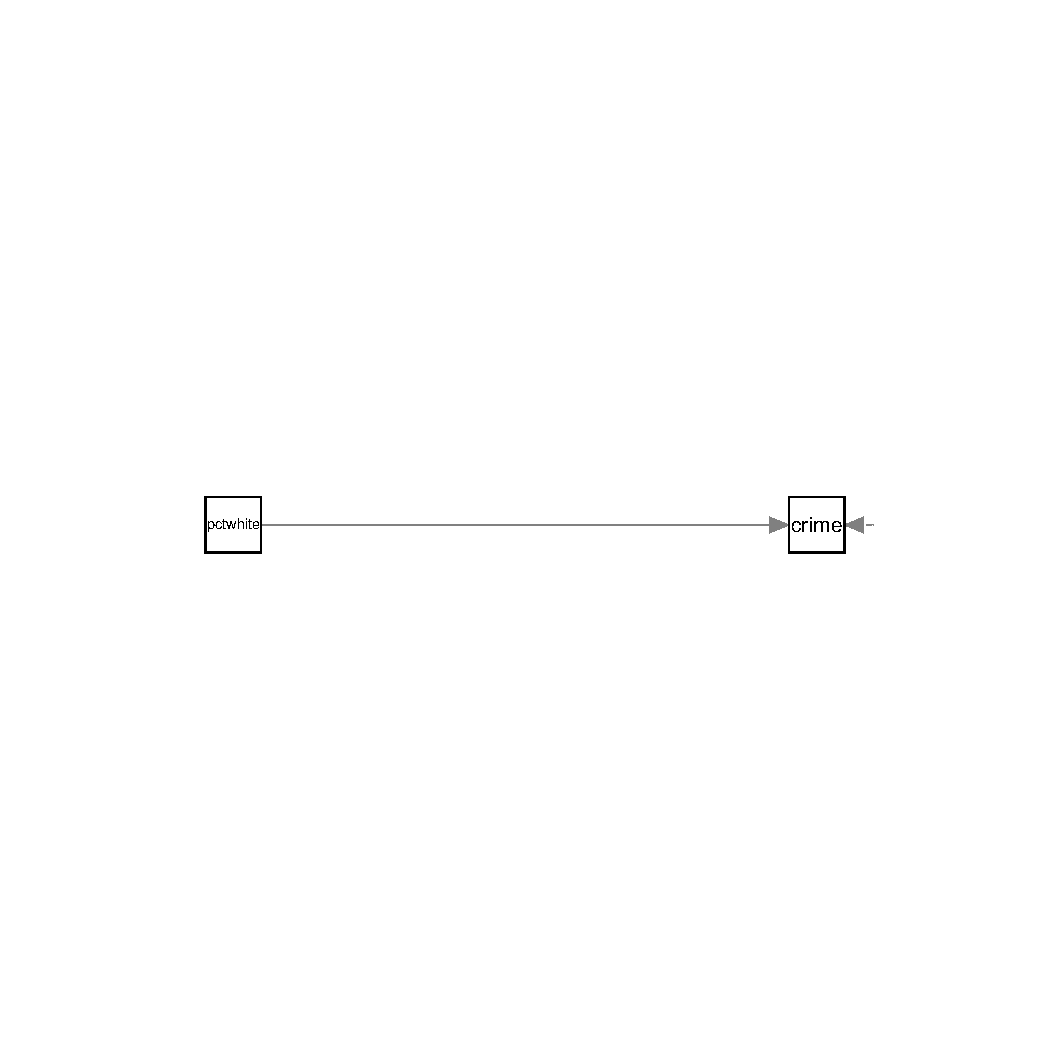
\includegraphics[width=\maxwidth]{figure/unnamed-chunk-4-1} 

\end{knitrout}

\subsection{Ergebnis berechnen und anfordern}
Um das Ergebnis zu erhalten, muss das Modell zuerst berechnet werden (\texttt{sem}), bevor es ausgegeben werden kann (\texttt{summary}). Befehle hierf\"ur:
\begin{itemize}
  \item \texttt{sem(model=MeinModell, data=Meinedaten)}
  \item \texttt{summary(ergebnisSem, std=TRUE, rsquare=TRUE)}
\end{itemize}

\begin{knitrout}
\definecolor{shadecolor}{rgb}{0.969, 0.969, 0.969}\color{fgcolor}\begin{kframe}
\begin{alltt}
\hlcom{# Berechnung der Modelle}
\hlstd{ergModelldirekt} \hlkwb{<-} \hlkwd{sem}\hlstd{(Modelldirekt,} \hlkwc{data} \hlstd{= crime_data)}
\end{alltt}


{\ttfamily\noindent\itshape\color{messagecolor}{\#\# Found more than one class "{}Model"{} in cache; using the first, from namespace 'lavaan'}}\begin{alltt}
\hlkwd{summary}\hlstd{(ergModelldirekt,} \hlkwc{std}\hlstd{=}\hlnum{TRUE}\hlstd{,} \hlkwc{rsquare}\hlstd{=}\hlnum{TRUE}\hlstd{)}
\end{alltt}
\begin{verbatim}
## lavaan (0.5-22) converged normally after   9 iterations
## 
##   Number of observations                            51
## 
##   Estimator                                         ML
##   Minimum Function Test Statistic                0.000
##   Degrees of freedom                                 0
## 
## Parameter Estimates:
## 
##   Information                                 Expected
##   Standard Errors                             Standard
## 
## Regressions:
##                    Estimate  Std.Err  z-value  P(>|z|)   Std.lv  Std.all
##   crime ~                                                               
##     pctwhite   (a)   -0.023    0.003   -6.572    0.000   -0.023   -0.052
## 
## Variances:
##                    Estimate  Std.Err  z-value  P(>|z|)   Std.lv  Std.all
##    .crime             0.103    0.020    5.050    0.000    0.103    0.541
## 
## R-Square:
##                    Estimate
##     crime             0.459
\end{verbatim}
\end{kframe}
\end{knitrout}

\subsection{Volles Modell erstellen und berechnen}
Das volle Modell enthält alle Pfade, drei insgesamt, d.h. alle Verbindungen zwischen den Prädiltoren und dem Kriterium sind eingezeichnet und werden auch berechnet.

Wie oben ausgeführt, sind das die Pfade a, b und c. Diese werden wieder mit der Tilde eingezeichnet.

Allerdings soll auch der indirekte Pfad berechnet werden, der ja aus 2 Komponenten besteht. Doppel- oder Mehrfachpfade werden nicht grundsätzlich berechnet, sondern müssen definiert und damit angefordert werden. Dafür muss dem Mehrfachpfad ein Name gegeben werden gefolgt von der Zeichenkombination \textbf{:=} (steht für: definiert durch) und anschließend den verwendeten Pfadnamen.
\begin{itemize}
  \item \textbf{indirekterPfad := Pfad*Pfad*Pfad...}
\end{itemize}
\begin{knitrout}
\definecolor{shadecolor}{rgb}{0.969, 0.969, 0.969}\color{fgcolor}\begin{kframe}
\begin{alltt}
\hlcom{# Modell 2: volles Modell}
\hlstd{Modellvoll} \hlkwb{<-} \hlstr{'crime ~ c*pctwhite # c Pfad direkt
               crime ~ b*pcths # b
               pcths ~ a*pctwhite # a

               indirekterPfad := a*b'} \hlcom{# Definition des ind. Pfads}

\hlstd{ergModellvoll} \hlkwb{<-} \hlkwd{sem}\hlstd{(Modellvoll,} \hlkwc{data} \hlstd{= crime_data)} \hlcom{# berechnen}

\hlkwd{summary}\hlstd{(ergModellvoll,} \hlkwc{std}\hlstd{=}\hlnum{TRUE}\hlstd{,} \hlkwc{rsquare}\hlstd{=}\hlnum{TRUE}\hlstd{)} \hlcom{# anzeigen}
\end{alltt}
\begin{verbatim}
## lavaan (0.5-22) converged normally after  19 iterations
## 
##   Number of observations                            51
## 
##   Estimator                                         ML
##   Minimum Function Test Statistic                0.000
##   Degrees of freedom                                 0
##   Minimum Function Value               0.0000000000000
## 
## Parameter Estimates:
## 
##   Information                                 Expected
##   Standard Errors                             Standard
## 
## Regressions:
##                    Estimate  Std.Err  z-value  P(>|z|)   Std.lv  Std.all
##   crime ~                                                               
##     pctwhite   (c)   -0.022    0.004   -6.095    0.000   -0.022   -0.051
##     pcths      (b)   -0.002    0.009   -0.277    0.782   -0.002   -0.030
##   pcths ~                                                               
##     pctwhite   (a)    0.143    0.056    2.569    0.010    0.143    0.026
## 
## Variances:
##                    Estimate  Std.Err  z-value  P(>|z|)   Std.lv  Std.all
##    .crime             0.103    0.020    5.050    0.000    0.103    0.541
##    .pcths            27.144    5.375    5.050    0.000   27.144    0.885
## 
## R-Square:
##                    Estimate
##     crime             0.459
##     pcths             0.115
## 
## Defined Parameters:
##                    Estimate  Std.Err  z-value  P(>|z|)   Std.lv  Std.all
##     indirekterPfad   -0.000    0.001   -0.275    0.783   -0.000   -0.001
\end{verbatim}
\begin{alltt}
\hlkwd{semPaths}\hlstd{(ergModellvoll,} \hlkwc{style}\hlstd{=}\hlstr{"lisrel"}\hlstd{,}\hlkwc{nCharNodes} \hlstd{=} \hlnum{0}\hlstd{,}
         \hlkwc{whatLabels}\hlstd{=}\hlstr{"std"}\hlstd{,}\hlkwc{intercepts} \hlstd{= F,}\hlkwc{rotation}\hlstd{=}\hlnum{2}\hlstd{)} \hlcom{# Graphik}
\end{alltt}
\end{kframe}
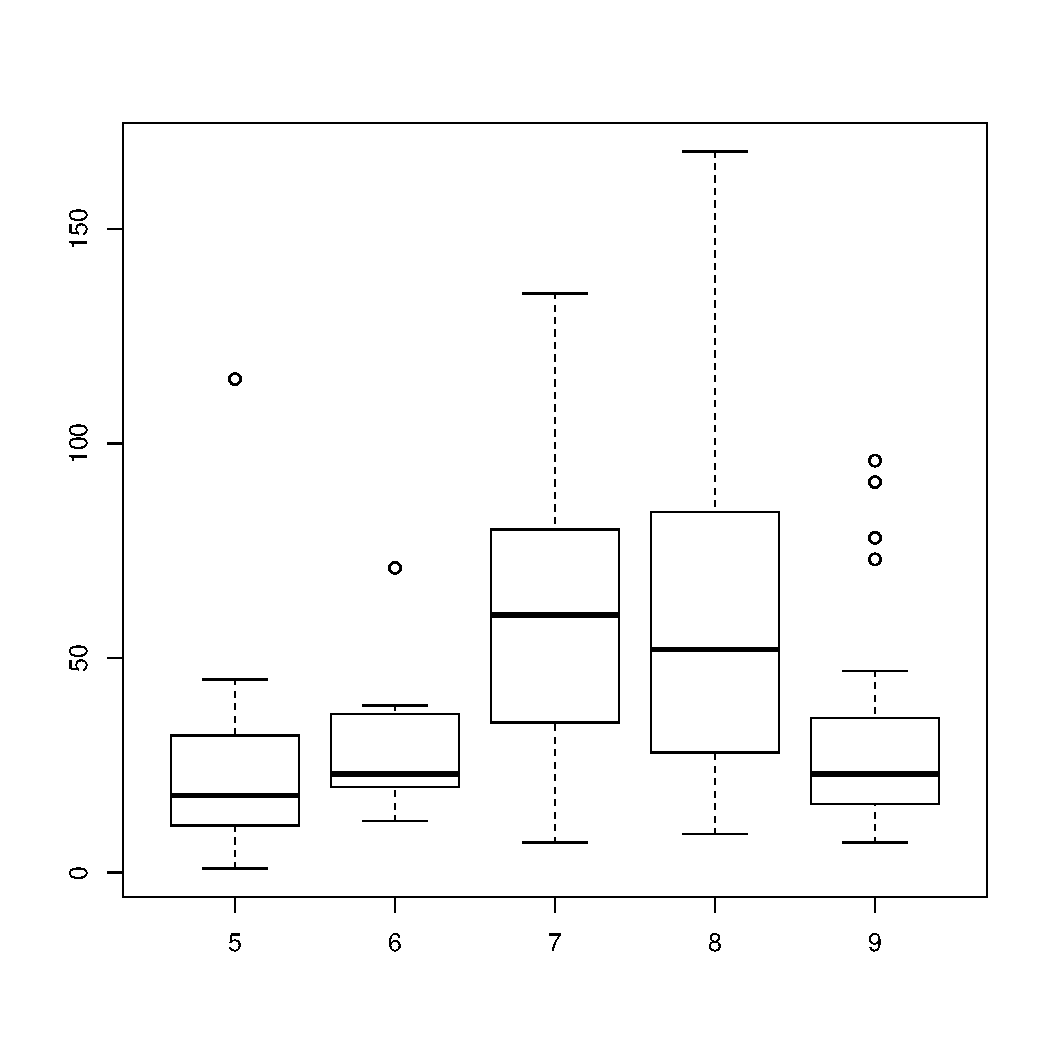
\includegraphics[width=\maxwidth]{figure/unnamed-chunk-6-1} 

\end{knitrout}


\subsection{indirektes Modell erstellen und berechnen}
Hierf\"ur braucht nicht mehr ein eigenes Modell erstellt werden (was möglich wäre), sondern es reicht, den Pfad c aus dem vollen Modell zu streichen. Das geschieht durch die Fixierung des Pfades auf 0.

Dazu reicht es, bei \textit{Berechnung des Modells} einen Befehl einzufügen: \textbf{constraints=' '} und innerhalb der Anführungszeichen den Pfadnamen aufzuführen gefolgt von 2 Gleichzeichen (heißt: weise den Wert zu) und 0.
\begin{knitrout}
\definecolor{shadecolor}{rgb}{0.969, 0.969, 0.969}\color{fgcolor}\begin{kframe}
\begin{alltt}
\hlstd{ergModellindirekt} \hlkwb{<-} \hlkwd{sem}\hlstd{(Modellvoll,} \hlkwc{data} \hlstd{= crime_data,}
                         \hlkwc{constraints}\hlstd{=}\hlstr{'c==0'}\hlstd{)} \hlcom{# Fixierung}

\hlkwd{summary}\hlstd{(ergModellindirekt,} \hlkwc{std}\hlstd{=}\hlnum{TRUE}\hlstd{,} \hlkwc{rsquare}\hlstd{=}\hlnum{TRUE}\hlstd{)} \hlcom{# Ergebnis}
\end{alltt}
\begin{verbatim}
## lavaan (0.5-22) converged normally after  15 iterations
## 
##   Number of observations                            51
## 
##   Estimator                                         ML
##   Minimum Function Test Statistic               27.908
##   Degrees of freedom                                 1
##   P-value (Chi-square)                           0.000
## 
## Parameter Estimates:
## 
##   Information                                 Observed
##   Standard Errors                             Standard
## 
## Regressions:
##                    Estimate  Std.Err  z-value  P(>|z|)   Std.lv  Std.all
##   crime ~                                                               
##     pctwhite   (c)    0.000       NA                      0.000    0.000
##     pcths      (b)   -0.020    0.011   -1.892    0.059   -0.020   -0.256
##   pcths ~                                                               
##     pctwhite   (a)    0.143    0.056    2.569    0.010    0.143    0.026
## 
## Variances:
##                    Estimate  Std.Err  z-value  P(>|z|)   Std.lv  Std.all
##    .crime             0.178    0.035    5.050    0.000    0.178    0.934
##    .pcths            27.144    5.375    5.050    0.000   27.144    0.885
## 
## R-Square:
##                    Estimate
##     crime             0.066
##     pcths             0.115
## 
## Defined Parameters:
##                    Estimate  Std.Err  z-value  P(>|z|)   Std.lv  Std.all
##     indirekterPfad   -0.003    0.002   -1.523    0.128   -0.003   -0.007
## 
## Constraints:
##                                                |Slack|
##     c - 0                                        0.000
\end{verbatim}
\end{kframe}
\end{knitrout}
Alternativ kann man die Fixierung auch direkt im Modell einzeichnen:
\begin{knitrout}
\definecolor{shadecolor}{rgb}{0.969, 0.969, 0.969}\color{fgcolor}\begin{kframe}
\begin{alltt}
\hlcom{# Modell 2: volles Modell}
\hlstd{Modellindirekt} \hlkwb{<-} \hlstr{'crime ~ c*pctwhite # c Pfad direkt
               crime ~ b*pcths # b
               pcths ~ a*pctwhite # a

               indirekterPfad := a*b # Definition des ind. Pfads
               c==0'} \hlcom{# der direkte Pfad wird so entfernt}

\hlstd{ergModellindirekt} \hlkwb{<-} \hlkwd{sem}\hlstd{(Modellindirekt,} \hlkwc{data} \hlstd{= crime_data)} \hlcom{# berechnen}

\hlkwd{summary}\hlstd{(ergModellindirekt,} \hlkwc{std}\hlstd{=}\hlnum{TRUE}\hlstd{,} \hlkwc{rsquare}\hlstd{=}\hlnum{TRUE}\hlstd{)} \hlcom{# Ergebnis}
\end{alltt}
\begin{verbatim}
## lavaan (0.5-22) converged normally after  15 iterations
## 
##   Number of observations                            51
## 
##   Estimator                                         ML
##   Minimum Function Test Statistic               27.908
##   Degrees of freedom                                 1
##   P-value (Chi-square)                           0.000
## 
## Parameter Estimates:
## 
##   Information                                 Expected
##   Standard Errors                             Standard
## 
## Regressions:
##                    Estimate  Std.Err  z-value  P(>|z|)   Std.lv  Std.all
##   crime ~                                                               
##     pctwhite   (c)    0.000    0.000    0.000    1.000    0.000    0.000
##     pcths      (b)   -0.020    0.011   -1.892    0.059   -0.020   -0.256
##   pcths ~                                                               
##     pctwhite   (a)    0.143    0.056    2.569    0.010    0.143    0.026
## 
## Variances:
##                    Estimate  Std.Err  z-value  P(>|z|)   Std.lv  Std.all
##    .crime             0.178    0.035    5.050    0.000    0.178    0.934
##    .pcths            27.144    5.375    5.050    0.000   27.144    0.885
## 
## R-Square:
##                    Estimate
##     crime             0.066
##     pcths             0.115
## 
## Defined Parameters:
##                    Estimate  Std.Err  z-value  P(>|z|)   Std.lv  Std.all
##     indirekterPfad   -0.003    0.002   -1.523    0.128   -0.003   -0.007
## 
## Constraints:
##                                                |Slack|
##     c - 0                                        0.000
\end{verbatim}
\end{kframe}
\end{knitrout}

\subsection{Vergleich von vollem und indirektem Modell}
Mit einem $\chi^{2}$ Differenztest kann man pr\"ufen, ob das indirekte Modell 'ausreicht', d.h. eine vollständige Mediation vorliegt.
\begin{knitrout}
\definecolor{shadecolor}{rgb}{0.969, 0.969, 0.969}\color{fgcolor}\begin{kframe}
\begin{alltt}
\hlkwd{anova}\hlstd{(ergModellvoll,ergModellindirekt)}
\end{alltt}
\begin{verbatim}
## Chi Square Difference Test
## 
##                   Df AIC BIC Chisq Chisq diff Df diff Pr(>Chisq)    
## ergModellvoll      0 759 769   0.0                                  
## ergModellindirekt  1 785 793  27.9       27.9       1    1.3e-07 ***
## ---
## Signif. codes:  0 '***' 0.001 '**' 0.01 '*' 0.05 '.' 0.1 ' ' 1
\end{verbatim}
\end{kframe}
\end{knitrout}


\end{document}
